% Layout extracted from Kupzyk report at ca1d062; retain a descriptive title.
\documentclass[11pt]{article}
\usepackage[letterpaper,margin=0.82in]{geometry}
\usepackage{booktabs,longtable,array,graphicx,amsmath,xcolor,hyperref,xurl}
\usepackage[authoryear,round]{natbib}
\hypersetup{colorlinks=true,urlcolor=blue,linkcolor=blue,citecolor=blue}
\renewcommand{\arraystretch}{1.25}
\setlength{\emergencystretch}{1em}
\setlength{\parskip}{5pt}\setlength{\parindent}{0pt}
% Use scalable fonts; inspect pdffonts output after building. Avoid adding T1
% fontenc without an installed scalable font family. Add title/date in manuscript.
\newcommand{\file}[2]{\href{https://github.com/alectionary/vibe-math/blob/master/formalization/denys-bosonic-pauli/#1}{\nolinkurl{#2}}}
\title{Phase choice and loss protection:\\A replication of Denys's bosonic Pauli codes}
\date{30 October 2026}
\begin{document}\maketitle
\begin{abstract}
We partly replicated the selected performance comparisons in Denys (2024), Figure~3.2: at seed amplitude $\alpha=1.5204$, changing the seed phase reduces entanglement infidelity by $0.0220613$ in the source and $0.0220613$ in our calculation, while enlarging the group raises it by $0.0011105$ and $0.0011030$, respectively. These four-amplitude results do not establish the full curve, its optimum, or agreement at the original solver's unknown numerical precision. Both source and reconstruction reverse the group ordering at $\alpha=2.0102$: enlargement lowers infidelity by $0.0004414$ and $0.0004552$, respectively; there is no source-to-replication sign reversal. Ten of twelve values lie inside deterministic figure-extraction envelopes obtained by perturbing marker and axis coordinates by $\pm0.05$ PDF points. Two extended-group values fall outside. An independent finite-photon calculation agrees with ours within $1.1\times10^{-8}$; the original implementation and solver uncertainty remain unresolved.
\end{abstract}
\begin{center}\small
\begin{tabular}{p{.27\linewidth}rrrr}
\toprule Claim at $\alpha=1.5204$ & Published & Ours & Same sign? & Verdict\\\midrule
Phase gain in infidelity & $+.0220613$ & $+.0220613$ & Yes & match\\
Group penalty in infidelity & $+.0011105$ & $+.0011030$ & Yes & partial\\
\bottomrule\end{tabular}\end{center}
{\small Source: marker extraction from \citet[p.~150, Fig.~3.2]{denys}; ours: recovery optimization. Positive phase gain favors the imaginary seed; positive group penalty disfavors enlargement. The phase-gain claim agrees in direction and lies within the extraction envelope; ``match'' is not a decimal-rounding verdict. The partial verdict retains a gap outside the extraction envelope. Original per-point precision and numerical uncertainty are unknown.}

\section{What replicated}
The selected performance comparisons partly replicate: at $\alpha=1.5204$, source and our phase gains are $.0220613$ and $.0220613$, and group penalties are $.0011105$ and $.0011030$. This is a bounded reconstruction, not a whole-dissertation replication or a measurement of optimal amplitude. No source-to-replication ordering reverses at any selected point; both show the group crossover. The comparison criterion is the $\pm.05$ PDF-point coordinate envelope, not a confidence interval or decimal-rounding rule.

Does increasing gate symmetry also improve loss protection? The seed phase matters greatly, but enlarging the group does not uniformly improve protection in this example. Denys's thesis, defended at Sorbonne Universit\'e on 5 April 2024 under Anthony Leverrier, constructs bosonic codes with covariant encodings. Chapter~3 fixes the encoding and optimizes recovery after independent pure loss $\gamma=.01$ in each of two modes \citep[pp.~148--151]{denys}. We check all three arms: the order-eight group $\langle X,Z\rangle$ with seeds $(\alpha,\alpha)$ (equal) and $(\alpha,i\alpha)$ (imaginary), and the order-sixteen group $\langle i,X,Z\rangle$ with seed $(\alpha,e^{i\pi/4}\alpha)$ (extended). Each seed specifies two coherent-state amplitudes; each code encodes one logical qubit.

The four amplitudes are exact common points on the inferred uniform source grid, $\alpha=.1+2.4k/49$ for $k=8,17,29,39$. They span the improvement region and crossover within a small computational budget; all three arms were run at each. This subset does not locate the true minimum. The source prose that enlargement ``appears to degrade'' protection is compatible with its better attainable minimum being worse even though the curves cross. We do not attribute a uniform pointwise ordering to that prose.

\begin{figure}[ht]\centering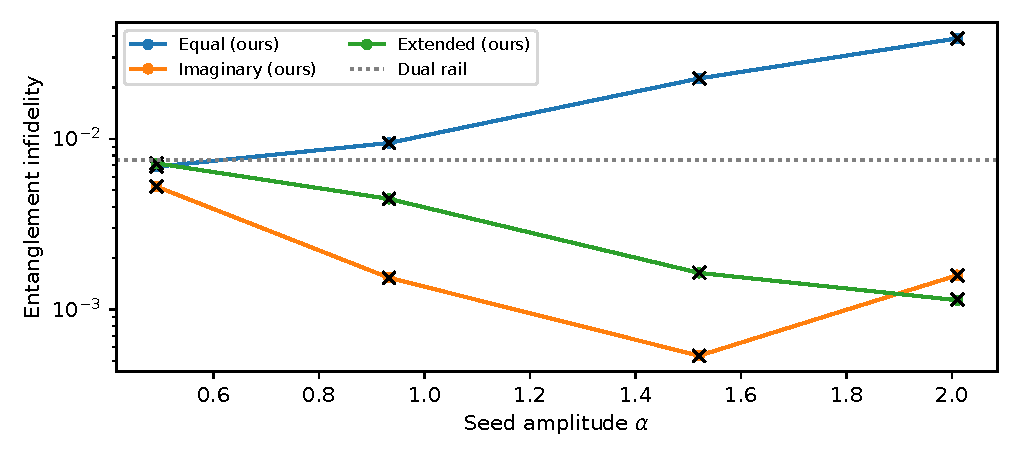
\includegraphics[width=.92\linewidth]{selected_performance.pdf}
\caption{Our infidelities (colored circles) and extracted source markers (black crosses) at twelve selected conditions. Source: Denys (2024), Figure~3.2. Lines only guide the eye; intermediate values were not computed. The horizontal line is our analytical dual-rail reference $3\gamma/4=.0075$.}\end{figure}

All declared signed comparisons preserve their source point directions. Phase gain is equal minus imaginary infidelity; group penalty is extended minus imaginary infidelity. Positive values respectively favor the imaginary phase and disfavor enlargement. The eight headline contrasts are below. Twelve supporting contrasts subtract dual-rail infidelity from each code's infidelity: positive means worse than dual rail. Both source and replication put imaginary and extended below dual rail at all four points, and equal below it only at the first. Full signed values and coverage are in \file{outputs/contrasts.json}{contrasts.json} and \file{outputs/coverage.json}{coverage.json}; they are separate from ours-minus-source deviations.
\begin{table}[ht]\centering\small
\begin{tabular}{lrrc}\toprule Amplitude / contrast & Source & Ours & Same sign?\\\midrule
0.492 / Phase gain & +0.0016148 & +0.0016154 & Yes \\
0.492 / Group penalty & +0.0019365 & +0.0019370 & Yes \\
0.933 / Phase gain & +0.0079242 & +0.0079242 & Yes \\
0.933 / Group penalty & +0.0029170 & +0.0029133 & Yes \\
1.520 / Phase gain & +0.0220613 & +0.0220613 & Yes \\
1.520 / Group penalty & +0.0011105 & +0.0011030 & Yes \\
2.010 / Phase gain & +0.0372244 & +0.0372313 & Yes \\
2.010 / Group penalty & -0.0004414 & -0.0004552 & Yes \\
\bottomrule
\end{tabular}
\caption{Headline contrasts in dimensionless infidelity. Source: extracted Figure~3.2 markers; ours: deterministic optimization. Unknown source solver uncertainty prevents an inferential source ranking.}\end{table}

\section{What we did ourselves, and what we took from others}
The original contribution is the encoding construction and reported loss comparison; ours is a bounded reconstruction and independent calculation. We use Denys's group-sum encoding, Eqs.~3.2 and 3.10, with $\Sigma=|0\rangle$, normalizing its columns in the coherent-state Gram matrix. The order-eight code reduces to odd/even cat products (Eqs.~3.60--3.61); the order-sixteen code additionally projects total photon number to $1$ modulo $4$. The source reading is recorded in \file{provenance/source_review.md}{source_review.md}.

The primary calculation has no photon-number cutoff. A finite coherent-state superposition remains in a finite coherent span after loss. For constellation amplitudes $z_k$, the channel maps
\[
 |z_k\rangle\langle z_l|\mapsto
 \langle\sqrt\gamma z_l|\sqrt\gamma z_k\rangle
 |\sqrt{1-\gamma}z_k\rangle\langle\sqrt{1-\gamma}z_l|.
\]
This equals the Kraus loss convention in Eq.~3.64. With logical block ordering, $H$ is one quarter of the encoded channel Choi matrix. We solve
\[
 F_{\rm opt}=\max_{J\succeq0}\operatorname{Tr}(HJ),\qquad J_{00}+J_{11}=I,
\]
where $J$ represents the adjoint recovery channel. Entanglement fidelity tests preservation of half of a normalized maximally entangled pair; plotted infidelity is $1-F_{\rm opt}$. Recovery optimization follows the established semidefinite framework of \citet{fletcher}. The channel and optimizer are \file{replicate.py\#L59}{replicate.py} and \file{replicate.py\#L75}{replicate.py}.

A different representation and solver independently confirm all twelve conditions. The check constructs photon-number parity states, applies binomial loss Kraus operators, compresses their image by singular-value decomposition, and separately assembles scalar recovery constraints. All SCS runs report optimal; the maximum primary--independent fidelity difference is $1.086\times10^{-8}$. Raising the photon cutoff from 32 to 40 and maximum total lost photons from 8 to 10 at the largest amplitude changes values by at most $5.43\times10^{-11}$. Shared inputs are the thesis definitions, objective and CVXPY frontend; this validates implementations and solvers, not an independently sourced experiment. See \file{independent_check.py}{independent_check.py}, \file{outputs/independent.json}{independent.json}, \file{outputs/independent_convergence.json}{independent_convergence.json}, and \file{provenance/computation_review.md}{computation_review.md}.

\section{What gave us trouble}
Ten numerical values fall inside source extraction envelopes and two fall outside. Every row below has limited reconstruction scope because original code and raw values were not obtained. Rounding verdicts are withheld for all twelve: the graph prints no per-point decimal precision. The displayed digits are our extraction format, not source reporting precision.
\begin{table}[ht]\centering\small
\begin{tabular}{lrrrr}\toprule Amplitude / code & Published estimate & Ours & Ours $-$ source & Envelope\\\midrule
0.492 / Equal & 0.006868100 & 0.006868089 & -1.19e-08 & inside \\
0.492 / Imaginary & 0.005253275 & 0.005252656 & -6.19e-07 & inside \\
0.492 / Extended & 0.007189816 & 0.007189624 & -1.92e-07 & inside \\
0.933 / Equal & 0.009458121 & 0.009458113 & -8.25e-09 & inside \\
0.933 / Imaginary & 0.001533936 & 0.001533936 & +7.37e-10 & inside \\
0.933 / Extended & 0.004450924 & 0.004447269 & -3.66e-06 & inside \\
1.520 / Equal & 0.022597000 & 0.022596979 & -2.02e-08 & inside \\
1.520 / Imaginary & 0.000535720 & 0.000535719 & -1.77e-10 & inside \\
1.520 / Extended & 0.001646173 & 0.001638760 & -7.41e-06 & outside \\
2.010 / Equal & 0.038812558 & 0.038819428 & +6.87e-06 & inside \\
2.010 / Imaginary & 0.001588115 & 0.001588114 & -1.49e-09 & inside \\
2.010 / Extended & 0.001146705 & 0.001132905 & -1.38e-05 & outside \\
\end{tabular}
\caption{Source: Figure~3.2 marker centers without interpolation. Ours: \file{outputs/primary.json}{primary.json}. For every row, precision is unavailable, numerical rounding verdict withheld, and scope limited. Envelope decisions refer only to extraction. Full endpoints: \file{outputs/comparison.json}{comparison.json}.}\end{table}

At $\alpha=1.520408$, extended has source estimate $.001646173$, extraction interval $[.001641278,.001651082]$, and our value $.001638760$: deviation $-7.413\times10^{-6}$. At $\alpha=2.010204$, the corresponding values are $.001146705$, $[.001143295,.001150125]$, and $.001132905$: deviation $-1.380\times10^{-5}$. Our numerical objective brackets, approximately $[.001638554,.001638760]$ and $[.001132903,.001132905]$, remain below those source intervals. These are discrepancies under our reading, not evidence of author error.

Optimizer warnings are retained. Nine primary solutions report optimal; three extended solutions at the first three amplitudes report optimal\_inaccurate. We did not replace these with the confirming solver's values. Positive-semidefinite and trace repairs give numerical primal/dual objective brackets, largest gap $2.063\times10^{-7}$. These floating-point feasibility diagnostics are not interval-arithmetic proofs. Independent agreement and endpoint tests support the scale of the differences despite warnings. Identity and complete-loss tests give fidelity 1 and $.25$; the dual-rail erasure model gives $.9925$. See \file{outputs/normalization.json}{normalization.json}.

\section{Assumptions}
\subsection{Inferred amplitude grid}
We infer the uniform grid $\alpha=.1+2.4k/49$ from marker positions, rather than from original plotting code. The largest horizontal residual is $.000184$ PDF points, supporting this interpretation. The four selected indices are present in every arm. This reconstruction assumption remains part of limited scope.
\subsection{Coordinate extraction envelope}
Each marker ordinate and each of two logarithmic axis coordinates may vary independently by $\pm.05$ PDF points. This conservative allowance exceeds the observed $.000184$-point grid-alignment residual; it does not bound original solver error. An independent reader extracted all146 markers before seeing our numerical results. Twelve common markers enter this replication. See \file{extract_source.py}{extract_source.py} and \file{source-evidence/source_values.json}{source_values.json}.
\subsection{Independent finite-photon approximation}
Only the independent calculation truncates photon number and lost photons. Its improved largest-amplitude check bounds encoding trace distance by $5.23\times10^{-13}$ and omitted-loss probability by $1.79\times10^{-19}$; these do not bound optimization error. Increasing the cutoff did not close either source gap. The primary coherent-span calculation has no such cutoff.
\subsection{Descriptive families without sampling inference}
The families are twelve source values, eight headline contrasts and twelve supporting contrasts. No Monte Carlo draws or seeds enter these deterministic calculations. There is no sampling alpha, multiplicity correction, or asserted unadjusted/adjusted confidence interval. Extraction bounds and our numerical brackets are separate from unknown source optimization uncertainty. The plan was recorded after pilot but before full-results review, not preregistered. No equivalence margin was selected. See \file{provenance/analysis_plan.json}{analysis_plan.json}.

\section{Ambiguities that were resolved}
\subsection{Fidelity versus infidelity}
The caption says fidelity, but the axis and nearby prose identify infidelity. The rendered \file{source-evidence/figure_3_2.png}{figure_3_2.png} resolves the quantity as $1-F$. This caption-label ambiguity is not a replication failure.
\subsection{Phase, group action and loss normalization}
Rendered equations fix conjugated group coefficients, parity order and square-root attenuation. Independent Fock construction and endpoint tests confirm these readings without closing the two gaps. Evidence: \file{source-evidence/pauli_states_eq_3_57_61.png}{pauli_states_eq_3_57_61.png}, \file{source-evidence/group_construction_eq_3_2.png}{group_construction_eq_3_2.png}, \file{source-evidence/bosonic_representation_eq_3_10.png}{bosonic_representation_eq_3_10.png}, and \file{source-evidence/pure_loss_eq_3_64.png}{pure_loss_eq_3_64.png}.
\subsection{Missing markers and the zero-amplitude reference}
The source contains 50 equal, 46 imaginary and 50 extended markers, starting at $\alpha=.1$. Missing imaginary indices 2,18,19,24 have no stated cause; they are not evidence of nonconvergence. We selected existing common points without imputation. The zero-amplitude dual-rail limit is an analytical reference, not an extracted marker. These boundary issues are not counted as replication failures.

\section{What remains unresolved}
Original solver settings are the leading unresolved explanation for the two gaps, but their cause is not established. Five candidates were checked. First, rendered and vector source extraction agree; both misses exceed the declared envelope. Second, scaling, phase and loss conventions agree across coherent and Fock formulations and pass endpoint tests. Third, a larger Fock cutoff moves values by less than $5.43\times10^{-11}$. Fourth, tight SCS agrees with the primary optimizer. Fifth, loose solver tolerances move extended-code infidelity substantially: at $\alpha=2.0102$, SCS tolerance $10^{-5}$ gives $.001175215$, versus $.001132904$ at $10^{-9}$. At $\alpha=1.5204$, tolerance $10^{-5}$ comes within $3.92\times10^{-7}$ of the source marker, but its feasibility violation and $3.04\times10^{-5}$ bracket make it an unreliable optimum. All sixteen diagnostic runs are retained in \file{outputs/solver_sensitivity.json}{solver_sensitivity.json}. Fitting a tolerance to a point would not recover the source procedure.

Unknown solver settings rank first because their measured effect exceeds the misses. Unrecorded implementation details rank second because the original Figure~3.2 program was not obtained, despite agreement of our two formulations. Coordinate error ranks lower within the declared envelope, which excludes our brackets. Original versions could not be matched: a thesis bibliography entry for SCS2.0.2 does not establish the actual Figure~3.2 runtime. No sampling noise, scored-instrument convention or statistical missing-data method applies. We stop at a bounded discrepancy under our reading. The decisive next artifact is the original Figure~3.2 generating bundle with unrounded points, solver versions, tolerances and residuals.

\section{Code and source availability}
The full thesis is readable from the author's GitHub repository, but original Figure~3.2 code and numerical output were not obtained. The dated search below distinguishes access denial from bounded negative search. The GitLab link concerns chapter2, not verified Figure~3.2 code. Limited attributed research excerpts are included without relicensing; the full thesis and third-party code are not distributed. See \file{provenance/availability.json}{availability.json} and \file{source-evidence/RIGHTS.md}{RIGHTS.md}.
\small\begin{longtable}{p{.23\linewidth}p{.13\linewidth}p{.56\linewidth}}\toprule Place & UTC date & Result\\\midrule\endhead
Author website / GitHub & 2026-10-30 & Full thesis read at 5aefd7b6caca97df7bf49ece36c6c91ba955d0fc. Only indexed public author repository; cloned and inspected. No chapter3 code or content license found. \\
Thesis code link / GitLab INRIA & 2026-10-30 & Related chapter2 code link. Web access denied by Anubis (9e4edb5b6b850c41); runtime policy excludes host. No bypass or runtime retry. Not evidence that chapter3 code is absent. \\
OSF & 2026-10-30 & Dated public web search for author and thesis/code terms found no relevant indexed artifact; bounded search, not proof of absence. \\
GitLab.com & 2026-10-30 & Dated public web search for author and thesis/code terms found no relevant indexed artifact; chapter2 link is on INRIA host. \\
Zenodo & 2026-10-30 & Dated public web search for author and thesis/code terms found no relevant indexed artifact. Original point data and solver settings not obtained. \\
\bottomrule
\end{longtable}\normalsize

\section{Next steps}
The original Figure~3.2 generating bundle would allow a replay at the two missed points, separating termination tolerances from implementation differences. A denser amplitude scan would address best attainable protection, a broader question than this reconstruction. No author outreach was performed.

\section{Compliance and software}
The approved layout is retained with a domain-specific engine departure. The following copied ledger corresponds to \file{provenance/compliance.json}{compliance.json}. Historical baseline and workflow are in \file{provenance/workflow.json}{workflow.json}: master \texttt{891774ca56c5}, skill revision \texttt{1e69e2c0e6fa}. The bundled approved preamble and latest Higgott paper preserve letter paper, .82-inch margins, 11-point text and 1.25 table spacing. Equations and deterministic uncertainty are subject-specific content adaptations.
\small\begin{longtable}{p{.23\linewidth}p{.12\linewidth}p{.57\linewidth}}\toprule Requirement & Status & Evidence / justification\\\midrule\endhead
Approved manuscript style & followed & Bundled preamble and latest Higgott narrative layout; no author line. Subject-specific equations and deterministic uncertainty replace Monte Carlo text. \\
Independent source and computation & followed & Source read separately; Fock/SCS check across all12; shared thesis and CVXPY declared. \\
Engine and preflight & departed & Accepted domain fallback; initial generic preflight rejected before compute, final validation recorded after compute. Justification: SEM engines do not represent quantum recovery SDP; independently validated CVXPY engines used. Accepted fallback recorded retrospectively. \\
Numerical precision and scope & followed & Rounding verdict withheld: plotted points have no printed decimal precision. All12 scope limited; extraction decisions separate. \\
Signed contrast inventory & followed & 8 headline and12 supporting contrasts; coverage check; zero point reversals. \\
Sampling and multiplicity & not applicable & Deterministic optimization: no Monte Carlo, alpha or inferential correction. Three descriptive families declared. \\
Source and software availability & followed & Five dated availability rows copied here; original code/settings unresolved. \\
Claim-to-source citations & followed & Thesis Fig3.2 and Eqs3.2,3.10,3.57--3.64 read directly; methodological abstracts/official package records verified; references used. \\
Evidence crops and rights & followed & 600dpi limited attributed crops; full thesis not bundled; third-party excerpts excluded from Apache grant. \\
Reproduction and delivery & followed & Saved-output rebuild separate from numerical reruns and external thesis extraction; immutable code revision recorded. Independent main-PDF review and remote hash record accompany PR. \\
\bottomrule
\end{longtable}\normalsize

Exact software versions and purposes are recorded. \href{https://github.com/python/cpython}{Python3.12.14} coordinates; \href{https://github.com/numpy/numpy}{NumPy2.3.5} and \href{https://github.com/scipy/scipy}{SciPy1.17.0} provide complex linear algebra. \href{https://github.com/cvxpy/cvxpy/tree/v1.7.3}{CVXPY1.7.3} expresses the SDP \citep{diamond}; \href{https://github.com/oxfordcontrol/Clarabel.rs/tree/v0.11.1}{Clarabel0.11.1} supplies the primary interior-point solver \citep{goulart}; \href{https://github.com/cvxgrp/scs}{SCS3.2.9} supplies a distinct operator-splitting solver \citep{odonoghue}. \href{https://github.com/pymupdf/PyMuPDF}{PyMuPDF1.26.6} reads vectors; \href{https://github.com/matplotlib/matplotlib}{Matplotlib3.10.8} plots. \href{https://gitlab.freedesktop.org/poppler/poppler}{Poppler26.05.0} renders evidence; \href{https://github.com/TeX-Live/texlive-source}{pdfTeX3.141592653-2.6-1.40.26}, TeX Live2025/dev/Debian, builds the paper. Pins and resources are in \file{requirements.txt}{requirements.txt} and \file{provenance/environment.json}{environment.json}. Method-reference metadata and relevant abstracts were checked against primary records; abstracts do not independently validate our derivation.

\appendix\section{Artifacts and reproduction}
Calculations and extraction are runnable at immutable commit \href{https://github.com/alectionary/vibe-math/tree/54ccd6bab1e53c31baccbce7745dff1eba44e743}{\nolinkurl{54ccd6bab1e53c31baccbce7745dff1eba44e743}}, which contains computational files and saved inputs. The later draft-PR artifact commit contains this manuscript. The historical master baseline is not the runnable target. File links point to master for navigation and will not resolve for new files until merge; use the PR's current-commit links before merge.

Exact commands, dependencies, working directory, expected outputs and overwrite behavior are in \file{README.md}{README.md}, subsections ``Rerun numerical calculations'', ``Rebuild the report from saved outputs'', and ``Re-extract the external source''. A saved-output rebuild needs neither thesis download nor optimization. Extraction requires the separately obtained hash-verified external thesis.
\small\begin{longtable}{p{.19\linewidth}p{.43\linewidth}p{.30\linewidth}}\toprule Claim & Files & Regeneration\\\midrule\endhead
Primary recovery & \file{replicate.py}{replicate.py}; \file{outputs/primary.json}{primary.json} & Run \texttt{replicate.py}; exact root-relative command in README\\
Independent check & \file{independent_check.py}{independent_check.py}; \file{outputs/independent.json}{independent.json} & Run \texttt{independent\_check.py}; larger-cutoff flags in README\\
Sensitivity & \file{diagnostics.py}{diagnostics.py}; \file{outputs/solver_sensitivity.json}{solver_sensitivity.json} & Run \texttt{diagnostics.py}\\
Tables/figure & \file{analyze.py}{analyze.py}; \file{paper/selected_performance.pdf}{selected_performance.pdf} & Run \texttt{analyze.py} on saved outputs\\
Source values & \file{extract_source.py}{extract_source.py}; \file{source-evidence/source_values.json}{source_values.json} & Run \texttt{extract\_source.py THESIS.pdf OUTDIR}\\
600dpi crops & \file{crop_source.py}{crop_source.py}; \file{source-evidence/crop_manifest.json}{crop_manifest.json} & Run \texttt{crop\_source.py THESIS.pdf OUTDIR}\\
Editable paper & \file{paper/phase_choice_and_loss_protection__a_replication_of_denys_pauli_codes.tex}{phase_choice_and_loss_protection__a_replication_of_denys_pauli_codes.tex}; \file{paper/references.tex}{references.tex} & Run \texttt{pdflatex} twice; exact filename in README\\
\bottomrule\end{longtable}\normalsize
\begin{thebibliography}{9}
\bibitem[Denys(2024)]{denys} Denys, A. (2024). \emph{Quantum key distribution and quantum error correction with bosonic systems}. Doctoral dissertation, Sorbonne Universit\'e. Defended 5 April 2024. \href{https://github.com/aurelie-denys/aurelie-denys.github.io/blob/5aefd7b6caca97df7bf49ece36c6c91ba955d0fc/PhDThesisAurelieDenys.pdf}{Author-hosted thesis, immutable source edition}.
\bibitem[Fletcher et al.(2007)]{fletcher} Fletcher, A.~S., Shor, P.~W., and Win, M.~Z. (2007). Optimum quantum error recovery using semidefinite programming. \emph{Physical Review A}, 75, 012338. \href{https://doi.org/10.1103/PhysRevA.75.012338}{doi:10.1103/PhysRevA.75.012338}.
\bibitem[Diamond and Boyd(2016)]{diamond} Diamond, S., and Boyd, S. (2016). CVXPY: A Python-embedded modeling language for convex optimization. \emph{Journal of Machine Learning Research}, 17(83), 1--5. \url{https://www.jmlr.org/papers/v17/15-408.html}.
\bibitem[Goulart and Chen(2024)]{goulart} Goulart, P.~J., and Chen, Y. (2024). Clarabel: An interior-point solver for conic programs with quadratic objectives. \href{https://arxiv.org/abs/2405.12762}{arXiv:2405.12762}.
\bibitem[O'Donoghue et al.(2016)]{odonoghue} O'Donoghue, B., Chu, E., Parikh, N., and Boyd, S. (2016). Conic optimization via operator splitting and homogeneous self-dual embedding. \emph{Journal of Optimization Theory and Applications}, 169(3), 1042--1068. \url{https://web.stanford.edu/~boyd/papers/scs.html}.
\end{thebibliography}

\end{document}
